\documentclass[a4,dvipdfmx,11pt]{article}


\usepackage{fancyhdr}
\usepackage{amsmath,amssymb}
\usepackage{fancybox,ascmac}
\usepackage[]{multicol}
\usepackage{caption}
\usepackage{mathtools}



\usepackage[dvipdfmx]{color}

\usepackage{float}
\usepackage[dvipdfmx]{graphicx}
\usepackage{tikz}
\usetikzlibrary{automata}
\usetikzlibrary{lindenmayersystems}
\usepackage{geometry}

\usepackage{amsthm}
\usepackage{amsmath}

\theoremstyle{definition}
\newtheorem{myth}{Theorem}[section]
\newtheorem{myproof}{Proof}[section]

\begin{document}

\section{Tunnel Troll Theorem}
\subsection{Introduction}
決定性Oritatami Systemでは転写されたbeadが固定される時、その位置は一意に定まる。
$\delta = 1$において転写されたbeadが一意に定まるためには、既に固定されている別のbeadとそのbeadがbondを結ぶか、あるいはトンネルを消費する必要がある。

ここで言う「トンネル」とは、ある三角格子上の点の周囲6点のうち、ちょうど4点が既に埋まっているような構造を指す。このトンネルの空いている頂点に直前のbeadが転写され、次のbeadがトンネルの中心に固定された時、そのbeadの周囲5点が埋まっていることになり、その次のbeadの位置は空いている1点に定まる。


この「トンネル」について以下が成り立つ。

\begin{myth}[Tunnel Troll Theorem]
  $|\Sigma| = 1, \delta = 1, \alpha = 2$を満たすOritatami Systemにおいて、トンネルを消費する時、Bondの数が減少する。
\end{myth}

\subsection{Proof}

この定理を示すには、トンネルを消費した際に増加するbondの数より減少するbondの数の方が多いことを示せば良い。


まず直前に固定されたbeadがトンネルの中にいるか外にいるかで場合分けを考える。トンネルの中にいる場合、次のbeadの固定される位置は既に決定されているが、次に固定される位置が再びトンネルの中であるかトンネルの外であるかでも場合分けを考える。また、トンネルの外にいる場合、そこがトンネルから離れた位置であるかトンネルの入り口であるかで場合分けをする(fig.\ref{TTT_position1})。パスは次のbeadが固定された時の状態遷移である。

\begin{figure}[h]
  \begin{center}
    \begin{tikzpicture}
      \draw[thick]
      (1.3,1)--(0,1)--(0,5)--(5,5)--(5,1)--(3.7,1);
      \node at(2.5,1) {トンネルの外};
      \node at (2.5,4) [rectangle, draw,rounded corners] (enter) {トンネルの入り口};
      \node at(2.5,2) [rectangle, draw, rounded corners] (outside) {トンネルから離れている};

      
      
      \draw[thick]
      (9.3,1)--(8,1)--(8,5)--(13,5)--(13,1)--(11.7,1);
      \node at(10.5,1) {トンネルの中};
      \node at(10.5,4) [rectangle, draw, rounded corners] (next-tunnel) {次もトンネル};
      \node at(10.5,2) [rectangle, draw, rounded corners] (next-outside) {次は外};

      \draw[->]
      (outside) edge [bend left] node[above] {} (enter)
                edge [loop left, transform canvas={xshift=-1cm}] node {} (outside)
      (enter)   edge [bend left] (next-tunnel)
                edge [bend left] (next-outside)
                edge [bend left] (outside)
      (next-tunnel) edge         (next-outside)
                edge [loop right]    (next-tunnel)
      (next-outside) edge[bend left] (outside)
                edge [bend left]     (enter)
      ;
      
    \end{tikzpicture}
    \caption{beadの位置による場合分け}
    \label{TTT_position1}
  \end{center}
\end{figure}

また、beadの位置とは別にトンネルの形状についても場合分けができる。三角格子上での対称性を考えるとトンネルの形状は以下の3つが考えられる(fig.\ref{TTT_tunnel})。この図において、バツが既にbeadが存在する頂点、白マルが空いている頂点である。また、トンネルの入口に注目すると、トンネルA,Bはどちらもトンネル内部に入る時のtranscriptのエッジに対して両側にbeadが存在する。一方でトンネルCは片側にのみbeadが存在する(fig.\ref{TTT_enterpoint})。出口についてはいずれのトンネルも同じ形になる(fig.\ref{TTT_exitpoint})。

\begin{figure}[h]
  \begin{center}
    \begin{tabular}{ccc}
      
      \begin{minipage}{0.3\hsize}
        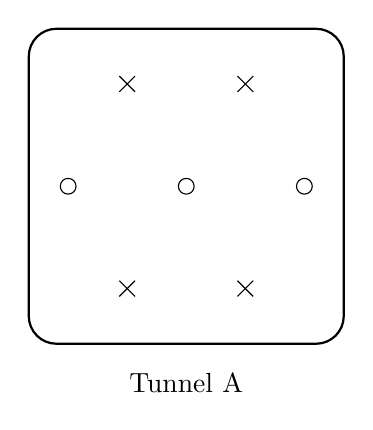
\begin{tikzpicture}
          \draw[thick, rounded corners = 10pt]
          (0,0)--(4,0)--(4,4)--(0,4)-- cycle;

          \begin{scope}[xshift=2cm, yshift=2cm]
            \draw(0,0) circle [radius=0.1];

            \foreach \theta in {0,180}{
              \draw[transform canvas={shift=(\theta:1.5)}](0,0) circle [radius=0.1];
            }
            
            \foreach \theta in {60,-60,120,-120}{
              \draw[transform canvas={shift=(\theta:1.5)}](-0.1,-0.1)--(0.1,0.1);
              \draw[transform canvas={shift=(\theta:1.5)}](0.1,-0.1)--(-0.1,0.1);
            }
          \end{scope}

          \node at (2,-0.5) {Tunnel A};
        \end{tikzpicture}
      \end{minipage}

      \begin{minipage}{0.3\hsize}
        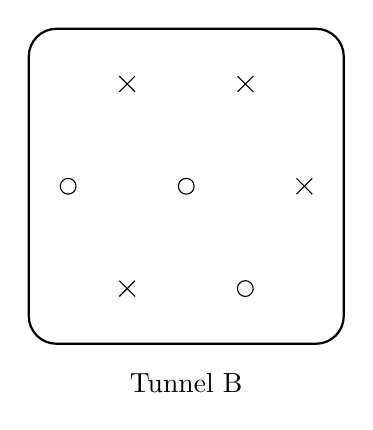
\begin{tikzpicture}
          \draw[thick, rounded corners = 10pt]
          (0,0)--(4,0)--(4,4)--(0,4)-- cycle;

          \begin{scope}[xshift=2cm, yshift=2cm]
            \draw(0,0) circle [radius=0.1];

            \foreach \theta in {-60,180}{
              \draw[transform canvas={shift=(\theta:1.5)}](0,0) circle [radius=0.1];
            }
            
            \foreach \theta in {0,60,120,-120}{
              \draw[transform canvas={shift=(\theta:1.5)}](-0.1,-0.1)--(0.1,0.1);
              \draw[transform canvas={shift=(\theta:1.5)}](0.1,-0.1)--(-0.1,0.1);
            }
          \end{scope}

          \node at (2,-0.5) {Tunnel B};
        \end{tikzpicture}
      \end{minipage}

      \begin{minipage}{0.3\hsize}
        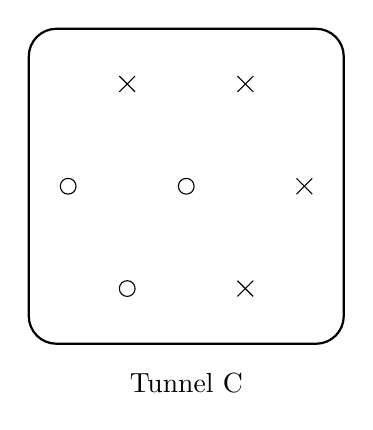
\begin{tikzpicture}
          \draw[thick, rounded corners = 10pt]
          (0,0)--(4,0)--(4,4)--(0,4)-- cycle;

          \begin{scope}[xshift=2cm, yshift=2cm]
            \draw(0,0) circle [radius=0.1];

            \foreach \theta in {-120,180}{
              \draw[transform canvas={shift=(\theta:1.5)}](0,0) circle [radius=0.1];
            }
            
            \foreach \theta in {0,60,-60,120}{
              \draw[transform canvas={shift=(\theta:1.5)}](-0.1,-0.1)--(0.1,0.1);
              \draw[transform canvas={shift=(\theta:1.5)}](0.1,-0.1)--(-0.1,0.1);
            }
          \end{scope}

          \node at (2,-0.5) {Tunnel C};
        \end{tikzpicture}
      \end{minipage}
      
    \end{tabular}
    \caption{トンネルの形状}
    \label{TTT_tunnel}
  \end{center}
\end{figure}

\begin{figure}[h]
  \begin{center}
    \begin{tabular}{cc}
      
      \begin{minipage}{0.45\hsize}
        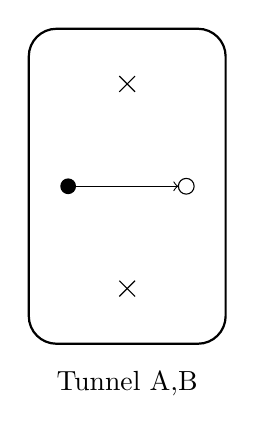
\begin{tikzpicture}
          \draw[thick, rounded corners = 10pt]
          (0,0)--(2.5,0)--(2.5,4)--(0,4)-- cycle;

          \begin{scope}[xshift=2cm, yshift=2cm]
            \draw(0,0) circle [radius=0.1];
            \fill[transform canvas={shift=(180:1.5)}](0,0) circle [radius=0.1];
            
            
            \foreach \theta in {120,-120}{
              \draw[transform canvas={shift=(\theta:1.5)}](-0.1,-0.1)--(0.1,0.1);
              \draw[transform canvas={shift=(\theta:1.5)}](0.1,-0.1)--(-0.1,0.1);
            }

            \draw[->] (-1.4,0) -- (-0.1,0);
          \end{scope}

          \node at (1.25,-0.5) {Tunnel A,B};
        \end{tikzpicture}
      \end{minipage}

      \begin{minipage}{0.45\hsize}
        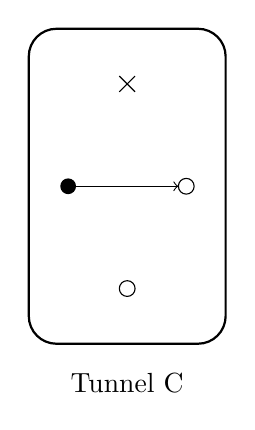
\begin{tikzpicture}
          \draw[thick, rounded corners = 10pt]
          (0,0)--(2.5,0)--(2.5,4)--(0,4)-- cycle;

          \begin{scope}[xshift=2cm, yshift=2cm]
            \draw(0,0) circle [radius=0.1];

            \draw[transform canvas={shift=(-120:1.5)}](0,0) circle [radius=0.1];
            \fill[transform canvas={shift=(180:1.5)}](0,0) circle [radius=0.1];
            
            
            \foreach \theta in {120}{
              \draw[transform canvas={shift=(\theta:1.5)}](-0.1,-0.1)--(0.1,0.1);
              \draw[transform canvas={shift=(\theta:1.5)}](0.1,-0.1)--(-0.1,0.1);
            }

            \draw[->] (-1.4,0) -- (-0.1,0);
          \end{scope}

          \node at (1.25,-0.5) {Tunnel C};
        \end{tikzpicture}
      \end{minipage}

    \end{tabular}
    \caption{トンネルの入り口}
    \label{TTT_enterpoint}
  \end{center}
\end{figure}

\begin{figure}[h]
  \begin{center}
    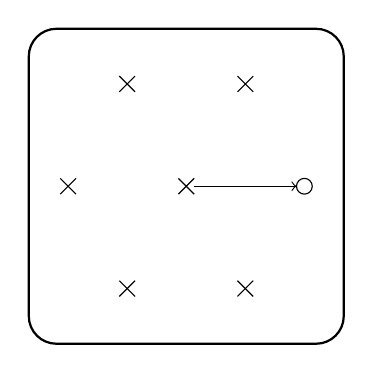
\begin{tikzpicture}
      \draw[thick, rounded corners = 10pt]
      (0,0)--(4,0)--(4,4)--(0,4)-- cycle;

      \begin{scope}[xshift=2cm, yshift=2cm]
        \draw[transform canvas={shift=(0:0)}](-0.1,-0.1)--(0.1,0.1);
        \draw[transform canvas={shift=(0:0)}](0.1,-0.1)--(-0.1,0.1);

        \foreach \theta in {0}{
          \draw[transform canvas={shift=(\theta:1.5)}](0,0) circle [radius=0.1];
        }
        
        \foreach \theta in {60,-60,120,-120,180}{
          \draw[transform canvas={shift=(\theta:1.5)}](-0.1,-0.1)--(0.1,0.1);
          \draw[transform canvas={shift=(\theta:1.5)}](0.1,-0.1)--(-0.1,0.1);
        }
        \draw[->] (0.1,0) -- (1.4,0);
      \end{scope}
    \end{tikzpicture}
    \caption{トンネルの出口}
    \label{TTT_exitpoint}
  \end{center}
\end{figure}

今、トンネルAとトンネルBの場合だけを考える。Appendixより、各状態遷移においてbondの増加量の最大値をそれぞれのedgeに加えると以下のようになる(fig.\ref{TTT_position2})。ただし$a$は自然数とし、「次は外」の状態に遷移するたびに値が更新される。この図のように、トンネルの内と外を往来するとbondの数が減少する。


次にトンネルCについて考える。fig.\ref{TTT_enterpoint}とfig.\ref{TTT_exitpoint}よりトンネルCの入口にbeadが固定される時、トンネルの出口とトンネルCの入口は共存出来ないため、トンネルCは連続したトンネル構造の途中や出口に使用することはできない。これを考慮し、トンネルCが使用されるケースについて場合分けを考える(fig.\ref{TTT_tunnelC_graph})。この場合分けの内、上2つはトンネルA,Bの中へ入るためbondの数が減少する。そのため下2つについて考えれば良い。Appendixより、いずれの場合もbondの数が減少する。



以上より、トンネルA,B,Cいずれを消費した場合も増加するbondの数より減少するbondの数の方が多い。よってこの定理は示された。


\begin{figure}[h]
  \begin{center}
    \begin{tikzpicture}
      \draw[thick]
      (1.3,1)--(0,1)--(0,5)--(5,5)--(5,1)--(3.7,1);
      \node at(2.5,1) {トンネルの外};
      \node at (2.5,4) [rectangle, draw,rounded corners] (enter) {トンネルの入り口};
      \node at(2.5,2) [rectangle, draw, rounded corners] (outside) {トンネルから離れている};

      
      
      \draw[thick]
      (9.3,1)--(8,1)--(8,5)--(13,5)--(13,1)--(11.7,1);
      \node at(10.5,1) {トンネルの中};
      \node at(10.5,4) [rectangle, draw, rounded corners] (next-tunnel) {次もトンネル};
      \node at(10.5,2) [rectangle, draw, rounded corners] (next-outside) {次は外};

      \draw[->]
      (outside) edge [bend left] node[left] {$-1$} (enter)
                edge [loop left, transform canvas={xshift=-1cm}] node[left] {$0$} (outside)
      (enter)   edge [bend left] node[above] {$-1$} (next-tunnel)
                edge [bend left] node[above] {$-a$} (next-outside)
                edge [bend left] node[right] {$0$}  (outside)
      (next-tunnel) edge         node[right] {$-a$} (next-outside)
                edge [loop right]node[right] {$0$}    (next-tunnel)
      (next-outside) edge[bend left] node[above] {$a$}  (outside)
                edge [bend left]     node[above] {$a-1$}(enter)
      ;
      
    \end{tikzpicture}
    \caption{Tunnel A,Bにおけるbondの増加量}
    \label{TTT_position2}
  \end{center}
\end{figure}

\begin{figure}[h]
  \begin{center}
    \begin{tikzpicture}
      \node at (0,4)   [rectangle, draw,rounded corners] (outside1) {トンネルから離れている};
      \node at (4.5,4) [rectangle, draw,rounded corners] (enter1)   {トンネルの入り口};
      \node at (8,4)   [rectangle, draw, rounded corners] (inside1) {トンネルC};
      \node at (11,4)  [rectangle, draw, rounded corners] (exit1)   {トンネルA,Bの中};
      \draw[->] (outside1)--(enter1);
      \draw[->] (enter1)  --(inside1);
      \draw[->] (inside1) --(exit1);
      
      
      \node at (0,3)   [rectangle, draw,rounded corners] (outside2) {トンネルの中};
      \node at (4.5,3) [rectangle, draw,rounded corners] (enter2)   {トンネルの入り口};
      \node at (8,3)   [rectangle, draw, rounded corners] (inside2) {トンネルC};
      \node at (11,3)  [rectangle, draw, rounded corners] (exit2)   {トンネルA,Bの中};     
      \draw[->] (outside2)--(enter2);
      \draw[->] (enter2)  --(inside2);
      \draw[->] (inside2) --(exit2);

      \node at (0,1)   [rectangle, draw,rounded corners] (outside3) {トンネルから離れている};
      \node at (4.5,1) [rectangle, draw,rounded corners] (enter3)   {トンネルの入り口};
      \node at (8,1)   [rectangle, draw, rounded corners] (inside3) {トンネルC};
      \node at (11,1)  [rectangle, draw, rounded corners] (exit3)   {トンネルの外};     
      \draw[->] (outside3)--(enter3);
      \draw[->] (enter3)  --(inside3);
      \draw[->] (inside3) --(exit3);

      \node at (0,0)   [rectangle, draw,rounded corners] (outside4) {トンネルの中};
      \node at (4.5,0) [rectangle, draw,rounded corners] (enter4)   {トンネルの入り口};
      \node at (8,0)   [rectangle, draw, rounded corners] (inside4) {トンネルC};
      \node at (11,0)  [rectangle, draw, rounded corners] (exit4)   {トンネルの外};     
      \draw[->] (outside4)--(enter4);
      \draw[->] (enter4)  --(inside4);
      \draw[->] (inside4) --(exit4);
    \end{tikzpicture}
    \caption{Tunnel Cの場合分け}
    \label{TTT_tunnelC_graph}
  \end{center}
\end{figure}

\newpage

\subsection{Appendix of Tunnel Troll Theorem}
\subsubsection{Entrance of TunnelA,B}
Tunnelの入口に固定されたbeadが、どの方向から来たかで場合分けをする(fig.\ref{TTT_tunnel_direction})。
その結果3通りの場合分けが出来るが、以下のようにいずれの場合もbondの総数は減少する。

\begin{itemize}
\item{Pattern1の時}\\
  四角で表されてる2頂点が埋まっているかどうかで分けられる。もしどちらも埋まっているとすると、トンネルの入り口ではなくトンネルの中になってしまうので、必ず少なくとも一方は空いている。今、頂点cが空いているとする。すると頂点Aの周囲は3点以上空いている事になる。Aの周囲2頂点はback boneとしてつながっている。そのためもしBが既にbondを消費しているならば、残りの1頂点に存在するbeadとのみbondを結ぶ事となる。頂点Bの周囲は3点空いている事を考えるとBは1つ以上のbondを残している。そのため入口に固定されるbeadと必ずbondを結ぶ事になる。もし頂点dも空いている場合、固定されるbeadはbondを2つとも消費し、かつ既存のbondも2つ消費しbondの総数は減少する。頂点dが埋まっていたとしても、頂点Aとは同様にしてbondを結び、決定的に固定するために頂点Bかdとbondを結ぶ。故にいずれの場合もbondの総数は減少する。

\item{Pattern2の時}\\
  Pattern1と同様にして頂点c,dが埋まっているかどうかで分けられる。Pattern1の例よりどちらも埋まっていることはない。頂点cが空いている場合決定的にbeadを固定するためにA,B少なくとも一方のbondを消費する。一方、頂点cが埋まっていて頂点dが空いている場合、Pattern1のように、固定されるbeadと頂点Bはbondを結ぶためbondを消費する。

  Pattern2の場合、固定されるbeadはbondを1つ増やす可能性がある。もし仮にbondが増えたとするならば、そのbondを使用するためはに頂点cかdにbeadが固定される必要がある。しかし今頂点BとPはback boneによってつながっている。Jordan curve theoremより、これ以降に転写され得るbeadの領域に頂点c,dは含まれないため、このbondを消費することはできず、bondの数は増加しない。よって既存のbondを減少させ、かつ新たに有効なbondを増やさないことからbondの総数は減少する。

\item{Pattern3の時}\\
  頂点nは空いているため、決定的に固定するために頂点c,d,eのいずれかとbondを結ぶ必要がある、そのため既存のbondを消費する。一方、固定されるbeadはbondを1つ増やす可能性があるが、pattern2と同様に頂点AとPがback boneでつながっているため、これ以降に転写され得るbeadの領域に頂点c,d,eは含まれていないため、増やされるbondを使用できない。よって既存のbondを減少させ、かつ新たに有効なbondを増やさないことからbondの総数は減少する。
  
\end{itemize}

\begin{figure}[h]
  \begin{center}
    \begin{tabular}{ccc}
      
      \begin{minipage}{0.3\hsize}
        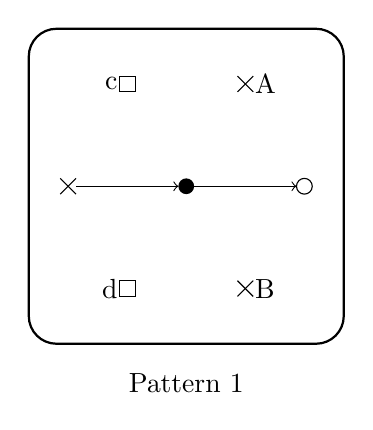
\begin{tikzpicture}
          \draw[thick, rounded corners = 10pt]
          (0,0)--(4,0)--(4,4)--(0,4)-- cycle;

          \begin{scope}[xshift=2cm, yshift=2cm]
            \fill(0,0) circle [radius=0.1];

            \foreach \theta in {0}{
              \draw[transform canvas={shift=(\theta:1.5)}](0,0) circle [radius=0.1];
            }
            
            \foreach \theta in {60,-60,180}{
              \draw[transform canvas={shift=(\theta:1.5)}](-0.1,-0.1)--(0.1,0.1);
              \draw[transform canvas={shift=(\theta:1.5)}](0.1,-0.1)--(-0.1,0.1);
            }

            \foreach \theta in {120,-120}{
              \draw[transform canvas={shift=(\theta:1.5)}](-0.1,-0.1) rectangle (0.1,0.1);
            }

            \draw[->] (180:1.4)--(180:0.1);
            \draw[->] (0:0.1)--(0:1.4);

            \node[transform canvas={shift=(60:1.5)},right] {A};
            \node[transform canvas={shift=(-60:1.5)},right] {B};

            \node[transform canvas={shift=(120:1.5)},left] {c};
            \node[transform canvas={shift=(-120:1.5)},left] {d};
          \end{scope}

          \node at (2,-0.5) {Pattern 1};
        \end{tikzpicture}
      \end{minipage}

      \begin{minipage}{0.3\hsize}
        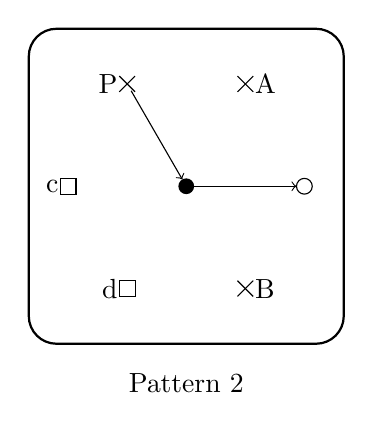
\begin{tikzpicture}
          \draw[thick, rounded corners = 10pt]
          (0,0)--(4,0)--(4,4)--(0,4)-- cycle;

          \begin{scope}[xshift=2cm, yshift=2cm]
            \fill(0,0) circle [radius=0.1];

            \foreach \theta in {0}{
              \draw[transform canvas={shift=(\theta:1.5)}](0,0) circle [radius=0.1];
            }
            
            \foreach \theta in {60,-60,120}{
              \draw[transform canvas={shift=(\theta:1.5)}](-0.1,-0.1)--(0.1,0.1);
              \draw[transform canvas={shift=(\theta:1.5)}](0.1,-0.1)--(-0.1,0.1);
            }

            \foreach \theta in {180,-120}{
              \draw[transform canvas={shift=(\theta:1.5)}](-0.1,-0.1) rectangle (0.1,0.1);
            }
            
            \draw[->] (120:1.4)--(120:0.1);
            \draw[->] (0:0.1)--(0:1.4);

            \node[transform canvas={shift=(60:1.5)},right] {A};
            \node[transform canvas={shift=(-60:1.5)},right] {B};
            \node[transform canvas={shift=(120:1.5)},left] {P};

            \node[transform canvas={shift=(180:1.5)},left] {c};
            \node[transform canvas={shift=(-120:1.5)},left] {d};
          \end{scope}

          \node at (2,-0.5) {Pattern 2};
        \end{tikzpicture}
      \end{minipage}

      \begin{minipage}{0.3\hsize}
        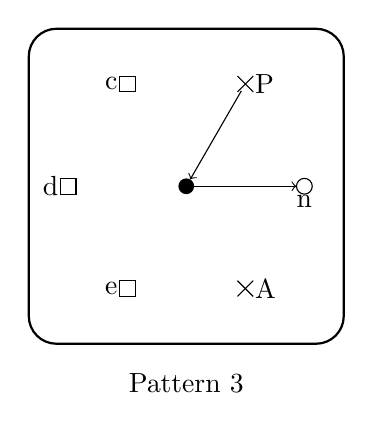
\begin{tikzpicture}
          \draw[thick, rounded corners = 10pt]
          (0,0)--(4,0)--(4,4)--(0,4)-- cycle;

          \begin{scope}[xshift=2cm, yshift=2cm]
            \fill(0,0) circle [radius=0.1];

            \foreach \theta in {0}{
              \draw[transform canvas={shift=(\theta:1.5)}](0,0) circle [radius=0.1];
            }
            
            \foreach \theta in {60,-60}{
              \draw[transform canvas={shift=(\theta:1.5)}](-0.1,-0.1)--(0.1,0.1);
              \draw[transform canvas={shift=(\theta:1.5)}](0.1,-0.1)--(-0.1,0.1);
            }

            \foreach \theta in {180,-120,120}{
              \draw[transform canvas={shift=(\theta:1.5)}](-0.1,-0.1) rectangle (0.1,0.1);
            }
            
            \draw[->] (60:1.4)--(60:0.1);
            \draw[->] (0:0.1)--(0:1.4);

            \node[transform canvas={shift=(-60:1.5)},right] {A};
            \node[transform canvas={shift=(60:1.5)},right] {P};

            \node[transform canvas={shift=(120:1.5)},left] {c};
            \node[transform canvas={shift=(180:1.5)},left] {d};
            \node[transform canvas={shift=(-120:1.5)},left] {e};
            \node[transform canvas={shift=(0:1.5)},below] {n};
          \end{scope}

          \node at (2,-0.5) {Pattern 3};
        \end{tikzpicture}
      \end{minipage}
      
    \end{tabular}
    \caption{入口へ至る方向}
    \label{TTT_tunnel_direction}
  \end{center}
\end{figure}


\subsubsection{Exit of Tunnel}

Tunnelの出口について場合分けを考える(fig.\ref{TTT_tunnel_exit})。この場合分けは頂点c,dについてその頂点が既に埋まっているか埋まっていないかで場合分けされている。なお、頂点c,dの両方とも埋まっている場合は、Tunnelの出口ではなくトンネルの中になるため場合分けに含めない。今、出口に固定されるbeadの1つ前のbeadが、$a$以下のbond消費したとする。すると以下で示されるようにTunnelの出口で増加するbondの数は高々$a$程度となる。つまり、Tunnelを出る事によって増加するbondの最大値は$0$となる。

\begin{itemize}
\item{Pattern1の時}\\
  頂点c,dが空いていたとする。入口の時と同様に考えると、頂点A,Bはbondを残しているため、頂点Pは頂点A,Bとbondを結ぶ。すなわち$a=2$となる。$\alpha = 2$を考えるとTunnel出口に固定されるbeadのよって増加するbondは高々$a=2$程度。
\item{Pattern2の時}\\
  頂点cのみが埋まっていたとする。頂点Bはbondを残しているため、頂点PとBはbondを結ぶ。よって$a \geq 1$また、Tunnel出口で固定されるbeadはbondを$2$増加させる可能性があるが、空いている頂点e,dについて一方はback boneとして消費されるため、このbeadが増加させたbondを使用できるのは後にbeadが頂点e,dのいずれかに来た時のみ。よってTunnel出口に固定されるbeadは有効なbondを高々$1$程度しか増やさない。よって増加するbondの数は高々$a$程度であることが言える。
  
\end{itemize}

\begin{figure}[h]
  \begin{center}
    \begin{tabular}{cc}
      
      \begin{minipage}{0.48\hsize}
        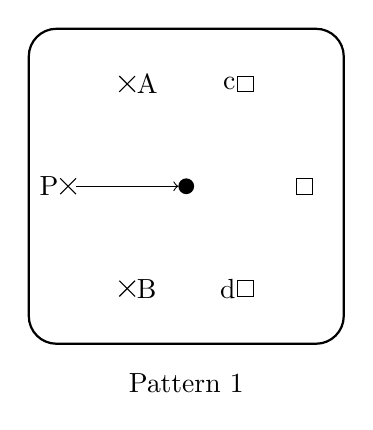
\begin{tikzpicture}
          \draw[thick, rounded corners = 10pt]
          (0,0)--(4,0)--(4,4)--(0,4)-- cycle;

          \begin{scope}[xshift=2cm, yshift=2cm]
            \fill(0,0) circle [radius=0.1];

            
            \foreach \theta in {120,-120,180}{
              \draw[transform canvas={shift=(\theta:1.5)}](-0.1,-0.1)--(0.1,0.1);
              \draw[transform canvas={shift=(\theta:1.5)}](0.1,-0.1)--(-0.1,0.1);
            }

            \foreach \theta in {0,60,-60}{
              \draw[transform canvas={shift=(\theta:1.5)}](-0.1,-0.1) rectangle (0.1,0.1);
            }

            \draw[->] (180:1.4)--(180:0.1);

            \node[transform canvas={shift=(120:1.5)},right] {A};
            \node[transform canvas={shift=(-120:1.5)},right] {B};
            \node[transform canvas={shift=(180:1.5)},left] {P};

            \node[transform canvas={shift=(60:1.5)},left] {c};
            \node[transform canvas={shift=(-60:1.5)},left] {d};
          \end{scope}

          \node at (2,-0.5) {Pattern 1};
        \end{tikzpicture}
      \end{minipage}

      \begin{minipage}{0.48\hsize}
        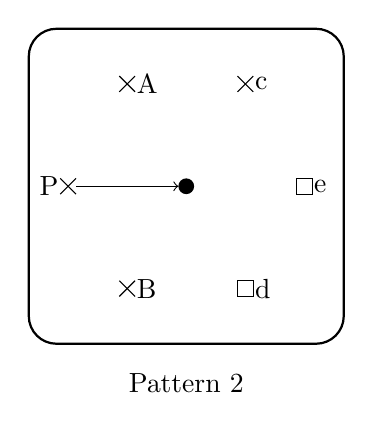
\begin{tikzpicture}
          \draw[thick, rounded corners = 10pt]
          (0,0)--(4,0)--(4,4)--(0,4)-- cycle;

          \begin{scope}[xshift=2cm, yshift=2cm]
            \fill(0,0) circle [radius=0.1];

            
            \foreach \theta in {120,-120,180,60}{
              \draw[transform canvas={shift=(\theta:1.5)}](-0.1,-0.1)--(0.1,0.1);
              \draw[transform canvas={shift=(\theta:1.5)}](0.1,-0.1)--(-0.1,0.1);
            }

            \foreach \theta in {0,-60}{
              \draw[transform canvas={shift=(\theta:1.5)}](-0.1,-0.1) rectangle (0.1,0.1);
            }

            \draw[->] (180:1.4)--(180:0.1);

            \node[transform canvas={shift=(120:1.5)},right] {A};
            \node[transform canvas={shift=(-120:1.5)},right] {B};
            \node[transform canvas={shift=(180:1.5)},left] {P};

            \node[transform canvas={shift=(-60:1.5)},right] {d};
            \node[transform canvas={shift=(60:1.5)},right] {c};
            \node[transform canvas={shift=(0:1.5)},right] {e};
          \end{scope}
          
          \node at (2,-0.5) {Pattern 2};
        \end{tikzpicture}
      \end{minipage}

      
      
    \end{tabular}
    \caption{出口のパターン}
    \label{TTT_tunnel_exit}
  \end{center}
\end{figure}


\subsubsection{Tunnel C}

Tunnel Cの入口に固定されるbeadについて、そのbeadがTunnelを消費して固定されたか、
そうでないかによって場合分けをする。なお、Tunnel Cの出口はTunnelA,Bの中でないとする。

\subsubsection{Tunnel Cの入口のbeadがTunnelを消費して固定された場合}
Tunnel Cの構造を維持したまま入口にTunnel消費によるbeadを固定するパターンはfig.\ref{TTT_tunnelC_enter_usingTunnel}の2通りがある。

\begin{itemize}
\item{Pattern1}\\
  頂点$t_1$が転写される前では、$t_3$がトンネルの外であることから頂点Aの周囲3点は空いてる。よって頂点Aのbeadは1つ以上bondを持つため、頂点Aと$t_1$はbondを結ぶ。また、頂点$t_2$が決定的に固定されるためには頂点B,C,Dとの間とbondを結ぶ必要がある。一方で、頂点$t_1,t_2$は、たとえbondを増やしたとしても周囲6点が埋まっているため、それを使うことができない。つまり$t_2$が固定された時点でbondは$2$減少している。今、$t_3$が固定された時を考えると、このbeadはbondを最大で2つ増やす可能性がある。しかし今$t_3$の周囲で空いているのは頂点e,fで、このうち一方はback boneのために使われるため、$t_3$の増やしたbondは1つのみが有効なbondとなる。よって全体でbondの総数を1以上減少させる。

\item{Pattern2}\\
  頂点$t_1$が固定される時そのbeadが幾つ周囲のbondを消費するかで場合分けできる。
  \begin{itemize}
  \item[-]{$t_1$がbondを消費しない場合}\\
    頂点$t_2$が決定的に固定される時、bondを1以上消費しかつ有効なbondを増やさない。頂点$t_3$が固定される時、頂点$t_1$はbondを持っているため、$t_3$,$t_1$の間でbondを結ぶ。よって$t_3$の固定で増加するbondの数は0以下。一方で、この時$t_1$はまだ有効なbondを一つ持っている。もし頂点eが埋まっているならこのbondは有効でなくなりbondの総数は減少する。そこで仮に頂点eが空いている場合を考える。今$t_3$の次に固定されるbeadを$t_4$とする。もし$t_4$が頂点eに固定されたなら、$t_1$のbondを消費しかつ$t_4$はbondを1つ消費し1つ増やす。よって$t_1$から$t_4$の固定においてbondの総数は減少する。次に$t_4$が頂点f,gのどちらかに固定される場合を考える。頂点eは空いているため、決定的に固定するに$t_4$は2つのbondを消費する必要がある。よって$t_1$が増やしたbondを加味してもbond$t_1$から$t_4$の固定でbondの総数を減らすことになる。よっていずれのケースを考えてもbondの総数は減少する。

  \item[-]{$t_1$がbondを1つ消費する場合}\\
    $t_2$は同様にしてbondの総数を1つ減少させ、$t_3$も増加させるbondの数は0以下。この時$t_1$はbondを増やさない。よってbondの総数は2以上減少する。
  \item[-]{$t_1$がbondを2つ消費する場合}\\
    $t_2$はbondを1つ以上減少させ、$t_3$はbondを2つ増加させる。よってbondの総数は減少する。
  \end{itemize}
\end{itemize}

\begin{figure}[h]
  \begin{center}
    \begin{tabular}{cc}
      
      \begin{minipage}{0.48\hsize}
        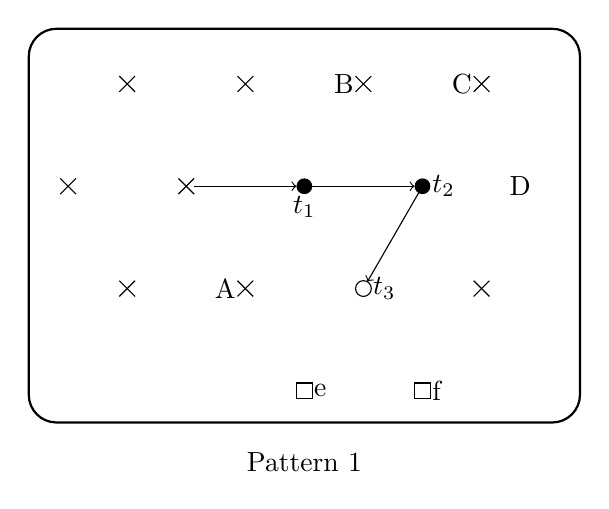
\begin{tikzpicture}
          \draw[thick, rounded corners = 10pt]
          (-2,2)--(5,2)--(5,-3)--(-2,-3)-- cycle;

          \draw[transform canvas={shift=(0:0)}](-0.1,-0.1)--(0.1,0.1);
          \draw[transform canvas={shift=(0:0)}](0.1,-0.1)--(-0.1,0.1);
          
          \foreach \theta in {60,-60,120,-120,180}{
            \draw[transform canvas={shift=(\theta:1.5)}](-0.1,-0.1)--(0.1,0.1);
            \draw[transform canvas={shift=(\theta:1.5)}](0.1,-0.1)--(-0.1,0.1);
          }

          \fill(0:1.5) circle [radius=0.1];
          \draw[->] (0:0.1)--(0:1.4);

          \node[left] at (-60:1.5) {A};

          \begin{scope}[shift=(0:3)]
            \fill(0,0) circle [radius=0.1];

            
            \foreach \theta in {120,60,-60}{
              \draw[transform canvas={shift=(\theta:1.5)}](-0.1,-0.1)--(0.1,0.1);
              \draw[transform canvas={shift=(\theta:1.5)}](0.1,-0.1)--(-0.1,0.1);
            }

            \draw[->] (180:1.4)--(180:0.1);
            \draw[->] (-120:0.1)--(-120:1.4);

            \node[below] at (180:1.5) {$t_1$};
            \node[right] at (0:0) {$t_2$};
            \node[right] at (-120:1.5) {$t_3$};

            \node[left] at (120:1.5) {B};
            \node[left] at (60:1.5) {C};
            \node[left] at (0:1.5) {D};

            \begin{scope}[shift=(-120:1.5)]
              \draw(0,0) circle [radius=0.1];
              \foreach \theta in {-120,-60}{
                \draw[transform canvas={shift=(\theta:1.5)}](-0.1,-0.1) rectangle (0.1,0.1);
              }

              \node[right] at (-120:1.5) {e};
              \node[right] at (-60:1.5) {f};
            \end{scope}
            
          \end{scope}

          \node at (1.5,-3.5) {Pattern 1};
        \end{tikzpicture}
      \end{minipage}

      \begin{minipage}{0.48\hsize}
        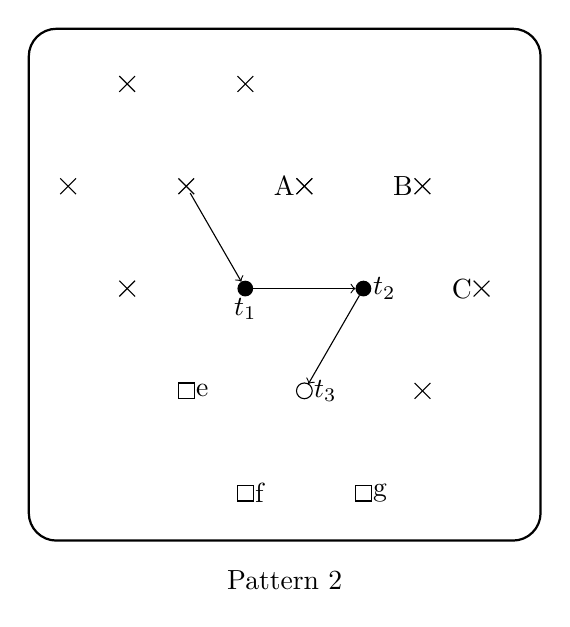
\begin{tikzpicture}
          \draw[thick, rounded corners = 10pt]
          (-2,2)--(4.5,2)--(4.5,-4.5)--(-2,-4.5)-- cycle;

          \draw[transform canvas={shift=(0:0)}](-0.1,-0.1)--(0.1,0.1);
          \draw[transform canvas={shift=(0:0)}](0.1,-0.1)--(-0.1,0.1);
          
          \foreach \theta in {60,0,120,-120,180}{
            \draw[transform canvas={shift=(\theta:1.5)}](-0.1,-0.1)--(0.1,0.1);
            \draw[transform canvas={shift=(\theta:1.5)}](0.1,-0.1)--(-0.1,0.1);
          }

          \draw[->] (-60:0.1)--(-60:1.4);


          \begin{scope}[shift=(-60:1.5),shift=(0:1.5)]
            \fill(0,0) circle [radius=0.1];
            \fill(180:1.5) circle [radius=0.1];

            
            \foreach \theta in {120,60,0,-60}{
              \draw[transform canvas={shift=(\theta:1.5)}](-0.1,-0.1)--(0.1,0.1);
              \draw[transform canvas={shift=(\theta:1.5)}](0.1,-0.1)--(-0.1,0.1);
            }

            \draw[->] (180:1.4)--(180:0.1);
            \draw[->] (-120:0.1)--(-120:1.4);

            \node[below] at (180:1.5) {$t_1$};
            \node[right] at (0:0) {$t_2$};
            \node[right] at (-120:1.5) {$t_3$};

            \node[left] at (120:1.5) {A};
            \node[left] at (60:1.5) {B};
            \node[left] at (0:1.5) {C};

            \begin{scope}[shift=(-120:1.5)]
              \draw(0,0) circle [radius=0.1];
              \foreach \theta in {180,-120,-60}{
                \draw[transform canvas={shift=(\theta:1.5)}](-0.1,-0.1) rectangle (0.1,0.1);
              }

              \node[right] at (180:1.5) {e};
              \node[right] at (-120:1.5) {f};
              \node[right] at (-60:1.5) {g};
            \end{scope}
            
          \end{scope}

          \node at (1.25,-5) {Pattern 2};
        \end{tikzpicture}
      \end{minipage}

      
      
    \end{tabular}
    \caption{Tunnelを消費して入口に固定されたbead}
    \label{TTT_tunnelC_enter_usingTunnel}
  \end{center}
\end{figure}

\end{document}
